\begin{tikzpicture}[scale=0.8,rotate=237]
    
    % Define los puntos de un triángulo.
    \tkzDefPoint(0,0){A}
    \tkzDefPoint(5,0){B}
    \tkzDefPoint(3,3){C}
    
    % Dibuja el triángulo
    \tkzDrawPolygon(A,B,C)

    %\tkzDrawPoints(A,B,C)
    \tkzLabelPoint[above](A){$P$}
    \tkzLabelPoint[left](B){$Q$}
    \tkzLabelPoint[right](C){$R$}
    
    % Marca cada lado con barras.
    \tkzMarkSegment[mark=|](A,B)
    \tkzMarkSegment[mark=||](B,C)
    \tkzMarkSegment[mark=|||](A,C)

    \tkzMarkAngle[arc=l,size=0.8](B,A,C)
    \tkzMarkAngle[arc=ll,size=0.8](C,B,A)
    \tkzMarkAngle[arc=lll,size=0.8](A,C,B)
    
\end{tikzpicture}